\chapter{Analisi dei requisiti}
\label{chap:analisi-requisiti}

\section{Analisi degli utenti}

Il sistema sviluppato nel contesto dello stage è un modulo di schedulazione C++ che espone la propria logica attraverso due interfacce principali: un'applicazione desktop basata su Qt (\texttt{erpai\_ui}), utilizzata per configurare, avviare e analizzare le pianificazioni durante lo sviluppo e il testing, e un server \gls{http} basato su Drogon (\texttt{erpai\_http}), attraverso cui il sistema gestionale \gls{erp} in PHP integra il solver in produzione.

Il sistema riconosce due attori:

\begin{itemize}
    \item \textbf{Operatore}: figura tecnica o semi-tecnica autorizzata a interagire con l'interfaccia Qt per configurare i parametri, avviare pianificazioni e analizzarne i risultati. È il soggetto principale della maggior parte dei casi d'uso descritti nel presente capitolo.
    \item \textbf{Sistema ERP}: applicazione PHP che, tramite l'API HTTP, avvia pianificazioni in modo automatizzato e ne ottiene i risultati senza intervento umano diretto. Partecipa esclusivamente alla specializzazione UC2.B dell'avvio pianificazione.
\end{itemize}

L'Operatore è tipicamente abituato a lavorare con strumenti gestionali e pannelli di monitoraggio. Di conseguenza l'interfaccia deve privilegiare chiarezza, immediatezza e coerenza tra le varie viste, in particolare nelle schermate di configurazione, di monitoraggio e di analisi del piano.

\section{Casi d'uso}

Per descrivere le funzionalità del sistema sono stati realizzati i relativi diagrammi dei casi d'uso. Un diagramma dei casi d'uso, in ambito \gls{uml}, permette di rappresentare le funzionalità offerte dal sistema e le interazioni che l'attore può avere con esse.

Nel seguito ogni caso d'uso corrisponde a un'azione distinta dell'Operatore. Le inclusioni (\textit{<<include>>}) sono utilizzate per raggruppare le sotto-attività obbligatorie e omogenee di uno stesso caso d'uso; le estensioni (\textit{<<extend>>}) descrivono esclusivamente scenari di errore o di deviazione dal flusso atteso; le specializzazioni modellano varianti alternative e mutuamente esclusive.

\begin{figure}[H]
    \centering
    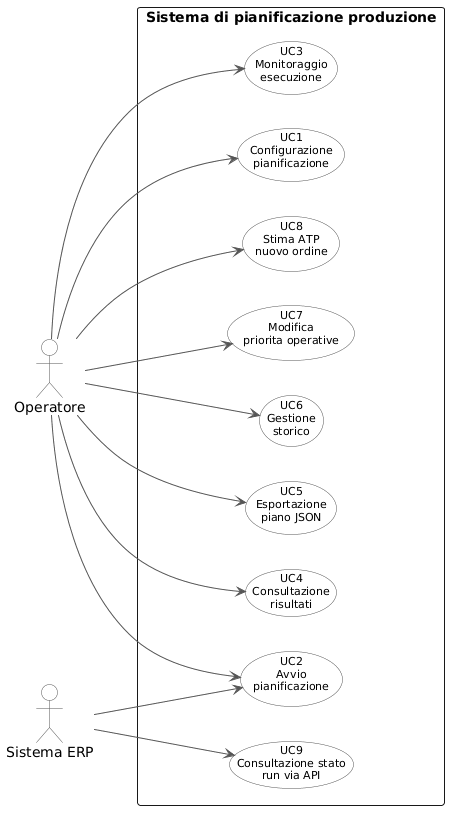
\includegraphics[width=0.65\columnwidth]{img/usecase/scenarioPrincipale.png}
    \caption{Scenario principale di utilizzo del sistema}
    \label{fig:scenario_principale}
\end{figure}

\subsection{Descrizione associata ai casi d'uso}

Ogni caso d'uso è descritto tramite un insieme di informazioni standard, riportate nella tabella seguente.

\begin{table}[H]
\centering
\renewcommand{\arraystretch}{1.2}
\begin{tabular}{|p{0.28\textwidth}|p{0.64\textwidth}|}
\hline
\rowcolor{tableGray}
\textbf{Campo} & \textbf{Descrizione} \\
\hline
Grafico UML & Rappresenta lo scenario del caso d'uso in oggetto. \\
\hline
Attore & Rappresenta la persona che interagisce con il sistema per avviare o consultare una funzionalità. \\
\hline
Scenario principale & Sequenza ordinata delle azioni compiute dall'Operatore per completare il caso d'uso. \\
\hline
Precondizioni & Condizioni che devono essere vere prima dell'esecuzione del caso d'uso. \\
\hline
Postcondizioni & Stato del sistema dopo il completamento corretto del caso d'uso. \\
\hline
Scenario alternativo & Flusso valido ma non principale, legato a un errore o a una deviazione dal comportamento atteso. \\
\hline
Inclusioni & Casi d'uso richiamati in modo obbligatorio dal caso d'uso corrente (\textit{<<include>>}). \\
\hline
Estensioni & Comportamenti condizionati, attivati solo al verificarsi di una situazione di errore (\textit{<<extend>>}). \\
\hline
Specializzazioni & Varianti mutuamente esclusive del caso d'uso generale. \\
\hline
Trigger & Evento o azione che avvia il caso d'uso. \\
\hline
\end{tabular}
\caption{Campi utilizzati per descrivere i casi d'uso.}
\label{tab:campi_casi_uso}
\end{table}

\subsection{Struttura gerarchica dei casi d'uso}

Le funzionalità del sistema sono organizzate nei seguenti casi d'uso.

\begin{itemize}
    \item \textbf{UC1 -- Configurazione pianificazione}
    \begin{itemize}
        \item UC1.1 -- Inserimento data di inizio pianificazione
        \item UC1.2 -- Inserimento timeout del solver
        \item UC1.3 -- Selezione strategia di risoluzione
        \item UC1.4 -- Selezione modalità di esecuzione del solver
    \end{itemize}

    \item \textbf{UC2 -- Avvio pianificazione}
    \begin{itemize}
        \item UC2.A -- Avvio da interfaccia Qt (specializzazione per Operatore)
        \item UC2.B -- Avvio da API HTTP (specializzazione per Sistema ERP)
    \end{itemize}

    \item \textbf{UC3 -- Monitoraggio esecuzione}
    \begin{itemize}
        \item UC3.1 -- Consultazione log di esecuzione
        \item UC3.2 -- Consultazione KPI in tempo reale
        \item UC3.3 -- Consultazione telemetria del solver
    \end{itemize}

    \item \textbf{UC4 -- Consultazione risultati}
    \begin{itemize}
        \item UC4.1 -- Visualizzazione diagramma di Gantt
        \item UC4.2 -- Visualizzazione task pianificati
        \item UC4.3 -- Analisi qualità del piano
    \end{itemize}

    \item \textbf{UC5 -- Esportazione piano in formato \gls{json}}

    \item \textbf{UC6 -- Gestione storico pianificazioni}
    \begin{itemize}
        \item UC6.1 -- Consultazione elenco storico pianificazioni
        \item UC6.2 -- Consultazione dettaglio esecuzione storica
    \end{itemize}

    \item \textbf{UC7 -- Modifica priorità operative}

    \item \textbf{UC8 -- Stima ATP per nuovo ordine}

    \item \textbf{UC9 -- Consultazione stato pianificazione via API}
\end{itemize}

\subsection{Dettaglio dei casi d'uso}

\subsubsection{Configurazione pianificazione}

\paragraph{UC1 -- Configurazione pianificazione}
\begin{itemize}
    \item \textbf{Attore principale:} Operatore.
    \item \textbf{Scenario principale:}
    \begin{enumerate}
        \item L'Operatore imposta la data di inizio della pianificazione $\rightarrow$ UC1.1.
        \item L'Operatore configura il timeout massimo del solver $\rightarrow$ UC1.2.
        \item L'Operatore seleziona la strategia di risoluzione da applicare $\rightarrow$ UC1.3.
        \item L'Operatore sceglie la modalità di esecuzione del solver $\rightarrow$ UC1.4.
    \end{enumerate}
    \item \textbf{Precondizioni:}
    \begin{itemize}
        \item l'applicazione è disponibile e raggiungibile.
        \item i dati di produzione necessari sono presenti nel database ERP.
    \end{itemize}
    \item \textbf{Postcondizioni:}
    \begin{itemize}
        \item i parametri risultano pronti per l'avvio della pianificazione.
    \end{itemize}
    \item \textbf{Inclusioni:}
    \begin{itemize}
        \item UC1.1 -- Inserimento data di inizio pianificazione.
        \item UC1.2 -- Inserimento timeout del solver.
        \item UC1.3 -- Selezione strategia di risoluzione.
        \item UC1.4 -- Selezione modalità di esecuzione del solver.
    \end{itemize}
    \item \textbf{Trigger:} l'Operatore vuole preparare una nuova esecuzione del solver.
\end{itemize}

\begin{figure}[H]
    \centering
    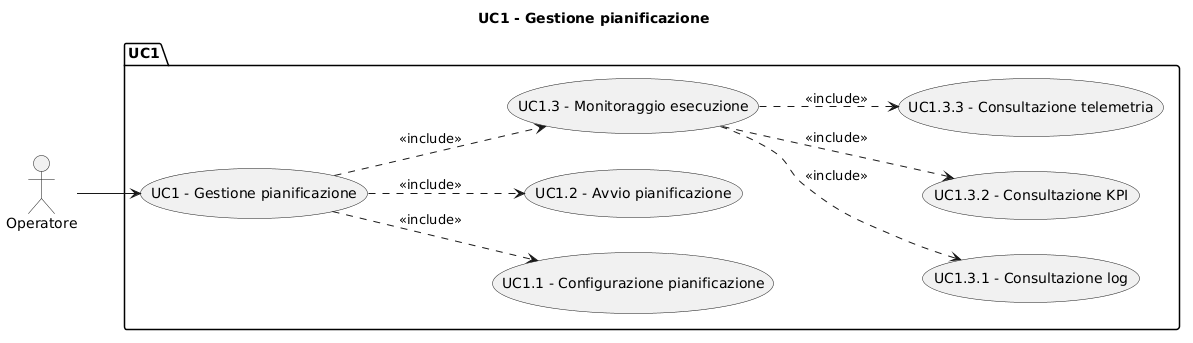
\includegraphics[width=0.85\columnwidth]{img/usecase/uc1.png}
    \caption{UC1 -- Configurazione pianificazione}
    \label{fig:uc1}
\end{figure}

\paragraph{UC1.1 -- Inserimento data di inizio pianificazione}
\begin{itemize}
    \item \textbf{Attore principale:} Operatore.
    \item \textbf{Scenario principale:}
    \begin{enumerate}
        \item L'Operatore accede al campo della data di inizio.
        \item L'Operatore seleziona o inserisce la data a partire dalla quale il solver deve collocare le attività.
    \end{enumerate}
    \item \textbf{Precondizioni:}
    \begin{itemize}
        \item l'applicazione è disponibile e raggiungibile.
        \item l'Operatore si trova nella schermata di configurazione $\rightarrow$ UC1.
    \end{itemize}
    \item \textbf{Postcondizioni:}
    \begin{itemize}
        \item la data di inizio risulta impostata nel form di configurazione.
    \end{itemize}
    \item \textbf{Trigger:} l'Operatore vuole definire il punto temporale di partenza della pianificazione.
\end{itemize}

\paragraph{UC1.2 -- Inserimento timeout del solver}
\begin{itemize}
    \item \textbf{Attore principale:} Operatore.
    \item \textbf{Scenario principale:}
    \begin{enumerate}
        \item L'Operatore accede al campo del timeout.
        \item L'Operatore inserisce il numero di secondi entro cui il solver deve produrre una soluzione.
    \end{enumerate}
    \item \textbf{Precondizioni:}
    \begin{itemize}
        \item l'applicazione è disponibile e raggiungibile.
        \item l'Operatore si trova nella schermata di configurazione $\rightarrow$ UC1.
    \end{itemize}
    \item \textbf{Postcondizioni:}
    \begin{itemize}
        \item il timeout risulta impostato nel form di configurazione.
    \end{itemize}
    \item \textbf{Trigger:} l'Operatore vuole definire il tempo massimo consentito alla fase di ottimizzazione.
\end{itemize}

\paragraph{UC1.3 -- Selezione strategia di risoluzione}
\begin{itemize}
    \item \textbf{Attore principale:} Operatore.
    \item \textbf{Scenario principale:}
    \begin{enumerate}
        \item L'Operatore accede al selettore della strategia di risoluzione.
        \item L'Operatore sceglie la strategia CP-SAT da applicare al problema di schedulazione.
    \end{enumerate}
    \item \textbf{Precondizioni:}
    \begin{itemize}
        \item l'applicazione è disponibile e raggiungibile.
        \item l'Operatore si trova nella schermata di configurazione $\rightarrow$ UC1.
    \end{itemize}
    \item \textbf{Postcondizioni:}
    \begin{itemize}
        \item la strategia risulta selezionata nel form di configurazione.
    \end{itemize}
    \item \textbf{Trigger:} l'Operatore vuole scegliere il metodo di risoluzione più adatto al contesto corrente.
\end{itemize}

\paragraph{UC1.4 -- Selezione modalità di esecuzione del solver}
\begin{itemize}
    \item \textbf{Attore principale:} Operatore.
    \item \textbf{Scenario principale:}
    \begin{enumerate}
        \item L'Operatore accede al selettore della modalità di esecuzione.
        \item L'Operatore sceglie se eseguire la fase di calcolo CP-SAT localmente oppure delegarla a un server remoto tramite gRPC.
    \end{enumerate}
    \item \textbf{Precondizioni:}
    \begin{itemize}
        \item l'applicazione è disponibile e raggiungibile.
        \item l'Operatore si trova nella schermata di configurazione $\rightarrow$ UC1.
    \end{itemize}
    \item \textbf{Postcondizioni:}
    \begin{itemize}
        \item la modalità di esecuzione risulta impostata nel form di configurazione.
    \end{itemize}
    \item \textbf{Trigger:} l'Operatore vuole decidere se delegare il calcolo a un server dedicato o eseguirlo localmente.
\end{itemize}

\subsubsection{Avvio pianificazione}

\paragraph{UC2 -- Avvio pianificazione}
\begin{itemize}
    \item \textbf{Attore principale:} Operatore (tramite interfaccia Qt) o Sistema ERP (tramite API HTTP).
    \item \textbf{Scenario principale:}
    \begin{enumerate}
        \item Il sistema riceve la richiesta di avvio.
        \item Il sistema carica i dati di produzione dal database ERP.
        \item Il sistema costruisce il modello CP-SAT e lo sottopone al solver.
        \item Il solver produce il piano di produzione.
        \item Il sistema rende il piano disponibile per la consultazione e registra l'esecuzione nello storico locale.
    \end{enumerate}
    \item \textbf{Precondizioni:}
    \begin{itemize}
        \item l'interfaccia di accesso è disponibile e raggiungibile.
        \item la configurazione è stata completata $\rightarrow$ UC1.
        \item il database ERP è accessibile e contiene dati di produzione validi.
    \end{itemize}
    \item \textbf{Postcondizioni:}
    \begin{itemize}
        \item il piano è stato generato e reso disponibile alle viste di consultazione.
        \item l'esecuzione è registrata nello storico locale con esito positivo.
    \end{itemize}
    \item \textbf{Scenario alternativo:} il solver restituisce una soluzione non ammissibile (stato \texttt{INFEASIBLE}) oppure viene interrotto per timeout senza aver trovato alcuna soluzione; il sistema registra l'errore nei log, aggiorna lo storico con esito negativo e non produce alcun piano.
    \item \textbf{Specializzazioni:}
    \begin{itemize}
        \item UC2.A -- Avvio da interfaccia Qt.
        \item UC2.B -- Avvio da API HTTP.
    \end{itemize}
    \item \textbf{Trigger:} l'Operatore o il Sistema ERP richiede il calcolo di una nuova soluzione di pianificazione.
\end{itemize}

\begin{figure}[H]
    \centering
    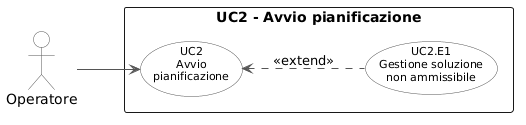
\includegraphics[width=0.7\columnwidth]{img/usecase/uc2.png}
    \caption{UC2 -- Avvio pianificazione}
    \label{fig:uc2}
\end{figure}

\paragraph{UC2.A -- Avvio da interfaccia Qt}
\begin{itemize}
    \item \textbf{Attore principale:} Operatore.
    \item \textbf{Scenario principale:}
    \begin{enumerate}
        \item L'Operatore preme il pulsante di avvio nell'interfaccia Qt.
        \item Il sistema esegue il flusso descritto in UC2.
        \item L'Operatore può seguire l'avanzamento in tempo reale tramite la vista di monitoraggio $\rightarrow$ UC3.
    \end{enumerate}
    \item \textbf{Precondizioni:}
    \begin{itemize}
        \item l'applicazione Qt è disponibile e raggiungibile.
        \item la configurazione è stata completata $\rightarrow$ UC1.
    \end{itemize}
    \item \textbf{Postcondizioni:}
    \begin{itemize}
        \item il piano è disponibile per la consultazione nell'interfaccia Qt $\rightarrow$ UC4.
    \end{itemize}
    \item \textbf{Trigger:} l'Operatore avvia manualmente la pianificazione dall'interfaccia grafica.
\end{itemize}

\paragraph{UC2.B -- Avvio da API HTTP}
\begin{itemize}
    \item \textbf{Attore principale:} Sistema ERP.
    \item \textbf{Scenario principale:}
    \begin{enumerate}
        \item Il Sistema ERP invia una richiesta HTTP POST all'endpoint \texttt{/api/planning/run} con i parametri della pianificazione: data di inizio, timeout, modalità di esecuzione del solver (\texttt{use\_remote\_solver}) e altri parametri avanzati facoltativi.
        \item Il server accetta la richiesta in modo asincrono e risponde immediatamente con HTTP 202 Accepted, restituendo un identificativo univoco del run (\texttt{run\_id}).
        \item Il sistema esegue il flusso descritto in UC2 in background.
        \item Il Sistema ERP utilizza il \texttt{run\_id} ricevuto per monitorare lo stato del run $\rightarrow$ UC9.
    \end{enumerate}
    \item \textbf{Precondizioni:}
    \begin{itemize}
        \item il server HTTP è disponibile e raggiungibile.
        \item il database ERP è accessibile e contiene dati di produzione validi.
    \end{itemize}
    \item \textbf{Postcondizioni:}
    \begin{itemize}
        \item il Sistema ERP ha ricevuto il \texttt{run\_id} e la pianificazione è in esecuzione in background.
        \item l'esecuzione sarà registrata nello storico locale al completamento.
    \end{itemize}
    \item \textbf{Trigger:} il Sistema ERP richiede automaticamente la pianificazione tramite l'API di produzione.
\end{itemize}

\subsubsection{Monitoraggio esecuzione}

\paragraph{UC3 -- Monitoraggio esecuzione}
\begin{itemize}
    \item \textbf{Attore principale:} Operatore.
    \item \textbf{Scenario principale:}
    \begin{enumerate}
        \item L'Operatore accede alla vista di monitoraggio.
        \item L'Operatore consulta i messaggi di log generati dal solver $\rightarrow$ UC3.1.
        \item L'Operatore consulta gli indicatori KPI aggiornati in tempo reale $\rightarrow$ UC3.2.
        \item L'Operatore consulta la telemetria dell'esecuzione $\rightarrow$ UC3.3.
    \end{enumerate}
    \item \textbf{Precondizioni:}
    \begin{itemize}
        \item l'applicazione è disponibile e raggiungibile.
        \item una pianificazione è in corso oppure i relativi dati di esecuzione sono disponibili $\rightarrow$ UC2.
    \end{itemize}
    \item \textbf{Postcondizioni:}
    \begin{itemize}
        \item l'Operatore dispone di un quadro aggiornato dello stato e dell'avanzamento della pianificazione.
    \end{itemize}
    \item \textbf{Inclusioni:}
    \begin{itemize}
        \item UC3.1 -- Consultazione log di esecuzione.
        \item UC3.2 -- Consultazione KPI in tempo reale.
        \item UC3.3 -- Consultazione telemetria del solver.
    \end{itemize}
    \item \textbf{Trigger:} l'Operatore desidera controllare lo stato di esecuzione del solver.
\end{itemize}

\begin{figure}[H]
    \centering
    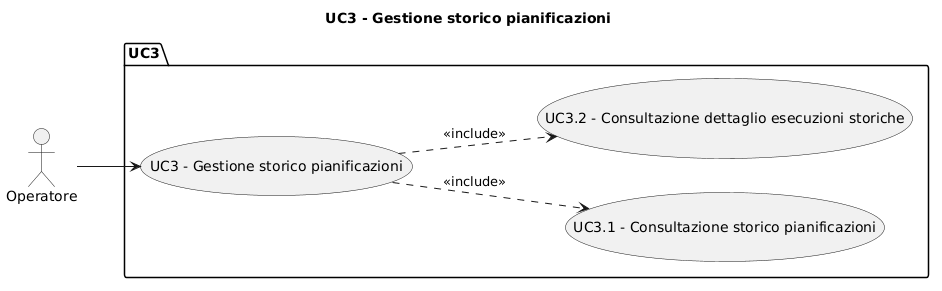
\includegraphics[width=0.85\columnwidth]{img/usecase/uc3.png}
    \caption{UC3 -- Monitoraggio esecuzione}
    \label{fig:uc3}
\end{figure}

\paragraph{UC3.1 -- Consultazione log di esecuzione}
\begin{itemize}
    \item \textbf{Attore principale:} Operatore.
    \item \textbf{Scenario principale:}
    \begin{enumerate}
        \item L'Operatore accede al pannello dei log.
        \item L'Operatore legge i messaggi informativi, di avviso o di errore generati durante l'esecuzione.
    \end{enumerate}
    \item \textbf{Precondizioni:}
    \begin{itemize}
        \item l'applicazione è disponibile e raggiungibile.
        \item una pianificazione è stata avviata o è stata completata.
        \item l'Operatore si trova nella vista di monitoraggio $\rightarrow$ UC3.
    \end{itemize}
    \item \textbf{Postcondizioni:}
    \begin{itemize}
        \item l'Operatore ha letto i log utili a comprendere l'esito o l'avanzamento dell'esecuzione.
    \end{itemize}
    \item \textbf{Trigger:} l'Operatore vuole verificare messaggi informativi, di avviso o di errore.
\end{itemize}

\paragraph{UC3.2 -- Consultazione KPI in tempo reale}
\begin{itemize}
    \item \textbf{Attore principale:} Operatore.
    \item \textbf{Scenario principale:}
    \begin{enumerate}
        \item L'Operatore accede alla sezione KPI.
        \item L'Operatore analizza gli indicatori di prestazione aggiornati: \gls{makespan}, \gls{lateness} totale e numero di task schedulati.
    \end{enumerate}
    \item \textbf{Precondizioni:}
    \begin{itemize}
        \item l'applicazione è disponibile e raggiungibile.
        \item il solver ha prodotto almeno un aggiornamento intermedio.
        \item l'Operatore si trova nella vista di monitoraggio $\rightarrow$ UC3.
    \end{itemize}
    \item \textbf{Postcondizioni:}
    \begin{itemize}
        \item l'Operatore ha valutato gli indicatori di qualità della soluzione corrente.
    \end{itemize}
    \item \textbf{Trigger:} l'Operatore vuole valutare l'efficienza del piano in corso di ottimizzazione.
\end{itemize}

\paragraph{UC3.3 -- Consultazione telemetria del solver}
\begin{itemize}
    \item \textbf{Attore principale:} Operatore.
    \item \textbf{Scenario principale:}
    \begin{enumerate}
        \item L'Operatore accede alla sezione telemetria.
        \item L'Operatore osserva l'andamento temporale dell'esecuzione, inclusi i valori di \gls{incumbent}, bound e gap forniti dal solver.
    \end{enumerate}
    \item \textbf{Precondizioni:}
    \begin{itemize}
        \item l'applicazione è disponibile e raggiungibile.
        \item il sistema sta eseguendo una pianificazione oppure ha già raccolto la telemetria di una sessione recente.
        \item l'Operatore si trova nella vista di monitoraggio $\rightarrow$ UC3.
    \end{itemize}
    \item \textbf{Postcondizioni:}
    \begin{itemize}
        \item l'Operatore dispone di un quadro dettagliato del comportamento interno del solver.
    \end{itemize}
    \item \textbf{Trigger:} l'Operatore desidera osservare l'evoluzione interna del processo di calcolo.
\end{itemize}

\subsubsection{Consultazione risultati}

\paragraph{UC4 -- Consultazione risultati}
\begin{itemize}
    \item \textbf{Attore principale:} Operatore.
    \item \textbf{Scenario principale:}
    \begin{enumerate}
        \item L'Operatore accede alla vista dei risultati.
        \item L'Operatore visualizza il diagramma di Gantt del piano $\rightarrow$ UC4.1.
        \item L'Operatore consulta l'elenco dei task pianificati $\rightarrow$ UC4.2.
        \item L'Operatore analizza la qualità del piano ottenuto $\rightarrow$ UC4.3.
    \end{enumerate}
    \item \textbf{Precondizioni:}
    \begin{itemize}
        \item l'applicazione è disponibile e raggiungibile.
        \item la pianificazione è stata completata con successo e ha prodotto un piano $\rightarrow$ UC2.
    \end{itemize}
    \item \textbf{Postcondizioni:}
    \begin{itemize}
        \item il piano è stato consultato nelle sue rappresentazioni principali.
    \end{itemize}
    \item \textbf{Inclusioni:}
    \begin{itemize}
        \item UC4.1 -- Visualizzazione diagramma di Gantt.
        \item UC4.2 -- Visualizzazione task pianificati.
        \item UC4.3 -- Analisi qualità del piano.
    \end{itemize}
    \item \textbf{Trigger:} l'Operatore vuole esaminare i risultati della schedulazione.
\end{itemize}

\begin{figure}[H]
    \centering
    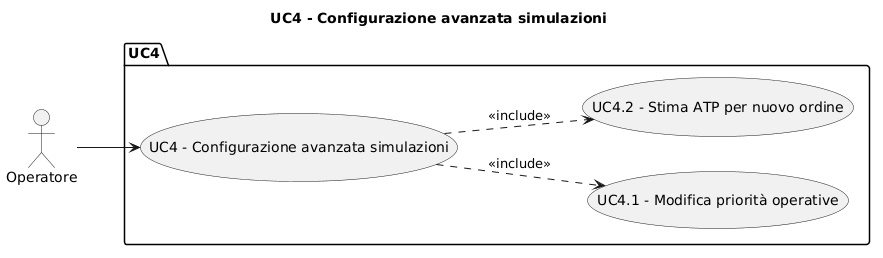
\includegraphics[width=0.85\columnwidth]{img/usecase/uc4.png}
    \caption{UC4 -- Consultazione risultati}
    \label{fig:uc4}
\end{figure}

\paragraph{UC4.1 -- Visualizzazione diagramma di Gantt}
\begin{itemize}
    \item \textbf{Attore principale:} Operatore.
    \item \textbf{Scenario principale:}
    \begin{enumerate}
        \item L'Operatore apre il pannello del diagramma di Gantt.
        \item L'Operatore analizza la distribuzione temporale dei task sulle macchine.
        \item L'Operatore legge le informazioni di dettaglio tramite i tooltip dei blocchi grafici.
    \end{enumerate}
    \item \textbf{Precondizioni:}
    \begin{itemize}
        \item l'applicazione è disponibile e raggiungibile.
        \item il piano di produzione è disponibile.
        \item l'Operatore si trova nella vista dei risultati $\rightarrow$ UC4.
    \end{itemize}
    \item \textbf{Postcondizioni:}
    \begin{itemize}
        \item l'Operatore ha valutato la sequenza temporale delle lavorazioni per macchina.
    \end{itemize}
    \item \textbf{Trigger:} l'Operatore vuole analizzare graficamente la distribuzione delle attività sulle risorse.
\end{itemize}

\paragraph{UC4.2 -- Visualizzazione task pianificati}
\begin{itemize}
    \item \textbf{Attore principale:} Operatore.
    \item \textbf{Scenario principale:}
    \begin{enumerate}
        \item L'Operatore apre la lista dei task pianificati.
        \item L'Operatore consulta gli attributi di ciascun task: macchina assegnata, orari di inizio e fine, quantità.
    \end{enumerate}
    \item \textbf{Precondizioni:}
    \begin{itemize}
        \item l'applicazione è disponibile e raggiungibile.
        \item il piano di produzione è stato calcolato.
        \item l'Operatore si trova nella vista dei risultati $\rightarrow$ UC4.
    \end{itemize}
    \item \textbf{Postcondizioni:}
    \begin{itemize}
        \item l'Operatore ha consultato i task schedulati dal solver.
    \end{itemize}
    \item \textbf{Trigger:} l'Operatore vuole verificare nel dettaglio il contenuto del piano.
\end{itemize}

\paragraph{UC4.3 -- Analisi qualità del piano}
\begin{itemize}
    \item \textbf{Attore principale:} Operatore.
    \item \textbf{Scenario principale:}
    \begin{enumerate}
        \item L'Operatore accede alla sezione di analisi qualità.
        \item L'Operatore esamina gli indicatori sintetici: makespan, lateness totale e numero di job in ritardo.
        \item L'Operatore verifica l'eventuale presenza di avvisi di validazione generati dal solver.
    \end{enumerate}
    \item \textbf{Precondizioni:}
    \begin{itemize}
        \item l'applicazione è disponibile e raggiungibile.
        \item un piano è stato generato ed è disponibile la relativa reportistica.
        \item l'Operatore si trova nella vista dei risultati $\rightarrow$ UC4.
    \end{itemize}
    \item \textbf{Postcondizioni:}
    \begin{itemize}
        \item l'Operatore ha una valutazione sintetica della bontà della soluzione prodotta.
    \end{itemize}
    \item \textbf{Trigger:} l'Operatore vuole valutare se il piano prodotto sia soddisfacente rispetto ai vincoli e agli obiettivi.
\end{itemize}

\subsubsection{Esportazione piano in formato JSON}

\paragraph{UC5 -- Esportazione piano in formato JSON}
\begin{itemize}
    \item \textbf{Attore principale:} Operatore.
    \item \textbf{Scenario principale:}
    \begin{enumerate}
        \item L'Operatore accede alla funzione di esportazione.
        \item L'Operatore seleziona il percorso di destinazione del file.
        \item Il sistema serializza il piano in formato JSON.
        \item Il file viene salvato su disco e il sistema notifica il completamento.
    \end{enumerate}
    \item \textbf{Precondizioni:}
    \begin{itemize}
        \item l'applicazione è disponibile e raggiungibile.
        \item il piano di produzione è disponibile $\rightarrow$ UC2.
    \end{itemize}
    \item \textbf{Postcondizioni:}
    \begin{itemize}
        \item il file JSON risulta disponibile all'Operatore nel percorso selezionato.
    \end{itemize}
    \item \textbf{Scenario alternativo:} la scrittura su disco fallisce per permessi insufficienti o spazio esaurito; il sistema notifica l'errore all'Operatore e il file non viene creato.
    \item \textbf{Trigger:} l'Operatore vuole ottenere una rappresentazione interoperabile del piano.
\end{itemize}

\begin{figure}[H]
    \centering
    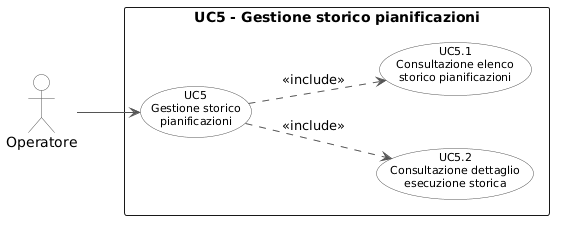
\includegraphics[width=0.65\columnwidth]{img/usecase/uc5.png}
    \caption{UC5 -- Esportazione piano in formato JSON}
    \label{fig:uc5}
\end{figure}

\subsubsection{Gestione storico pianificazioni}

\paragraph{UC6 -- Gestione storico pianificazioni}
\begin{itemize}
    \item \textbf{Attore principale:} Operatore.
    \item \textbf{Scenario principale:}
    \begin{enumerate}
        \item L'Operatore apre la sezione storico e consulta l'elenco delle pianificazioni precedenti $\rightarrow$ UC6.1.
        \item L'Operatore seleziona una pianificazione dall'elenco e ne consulta il dettaglio $\rightarrow$ UC6.2.
    \end{enumerate}
    \item \textbf{Precondizioni:}
    \begin{itemize}
        \item l'applicazione è disponibile e raggiungibile.
        \item lo storico locale contiene almeno una pianificazione memorizzata.
    \end{itemize}
    \item \textbf{Postcondizioni:}
    \begin{itemize}
        \item l'Operatore ha consultato i dati storici delle pianificazioni precedenti.
    \end{itemize}
    \item \textbf{Inclusioni:}
    \begin{itemize}
        \item UC6.1 -- Consultazione elenco storico pianificazioni.
        \item UC6.2 -- Consultazione dettaglio esecuzione storica.
    \end{itemize}
    \item \textbf{Trigger:} l'Operatore vuole confrontare esecuzioni passate o recuperare informazioni pregresse.
\end{itemize}

\begin{figure}[H]
    \centering
    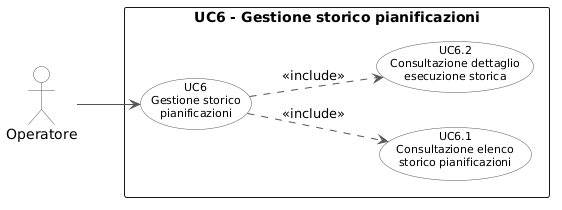
\includegraphics[width=0.75\columnwidth]{img/usecase/uc6.png}
    \caption{UC6 -- Gestione storico pianificazioni}
    \label{fig:uc6}
\end{figure}

\paragraph{UC6.1 -- Consultazione elenco storico pianificazioni}
\begin{itemize}
    \item \textbf{Attore principale:} Operatore.
    \item \textbf{Scenario principale:}
    \begin{enumerate}
        \item L'Operatore apre la sezione storico.
        \item L'Operatore scorre l'elenco delle pianificazioni precedenti e ne consulta i dati principali: data, durata e stato dell'esecuzione.
    \end{enumerate}
    \item \textbf{Precondizioni:}
    \begin{itemize}
        \item l'applicazione è disponibile e raggiungibile.
        \item lo storico locale contiene almeno una pianificazione memorizzata.
        \item l'Operatore si trova nella sezione storico $\rightarrow$ UC6.
    \end{itemize}
    \item \textbf{Postcondizioni:}
    \begin{itemize}
        \item l'Operatore ha consultato l'elenco delle esecuzioni passate.
    \end{itemize}
    \item \textbf{Trigger:} l'Operatore vuole accedere allo storico delle pianificazioni eseguite.
\end{itemize}

\paragraph{UC6.2 -- Consultazione dettaglio esecuzione storica}
\begin{itemize}
    \item \textbf{Attore principale:} Operatore.
    \item \textbf{Scenario principale:}
    \begin{enumerate}
        \item L'Operatore seleziona una pianificazione dall'elenco storico $\rightarrow$ UC6.1.
        \item L'Operatore visualizza il dettaglio dell'esecuzione: esito, KPI, log e task pianificati.
    \end{enumerate}
    \item \textbf{Precondizioni:}
    \begin{itemize}
        \item l'applicazione è disponibile e raggiungibile.
        \item esiste almeno una pianificazione storica selezionabile.
        \item l'Operatore sta consultando l'elenco storico $\rightarrow$ UC6.1.
    \end{itemize}
    \item \textbf{Postcondizioni:}
    \begin{itemize}
        \item il dettaglio della specifica esecuzione storica è stato consultato.
    \end{itemize}
    \item \textbf{Trigger:} l'Operatore vuole approfondire i dati di una singola esecuzione passata.
\end{itemize}

\subsubsection{Modifica priorità operative}

\paragraph{UC7 -- Modifica priorità operative}
\begin{itemize}
    \item \textbf{Attore principale:} Operatore.
    \item \textbf{Scenario principale:}
    \begin{enumerate}
        \item L'Operatore accede alla sezione delle priorità operative.
        \item L'Operatore modifica i valori di priorità da applicare alla logica di pianificazione.
        \item Il sistema aggiorna i parametri per le elaborazioni successive.
    \end{enumerate}
    \item \textbf{Precondizioni:}
    \begin{itemize}
        \item l'applicazione è disponibile e raggiungibile.
        \item il sistema consente la modifica dei parametri di priorità.
    \end{itemize}
    \item \textbf{Postcondizioni:}
    \begin{itemize}
        \item le nuove priorità risultano pronte per essere applicate alla pianificazione successiva.
    \end{itemize}
    \item \textbf{Trigger:} l'Operatore desidera adattare la logica di schedulazione alle necessità operative correnti.
\end{itemize}

\begin{figure}[H]
    \centering
    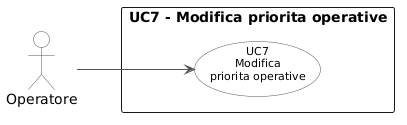
\includegraphics[width=0.75\columnwidth]{img/usecase/uc7.png}
    \caption{UC7 -- Modifica priorità operative}
    \label{fig:uc7}
\end{figure}

\subsubsection{Stima ATP per nuovo ordine}

\paragraph{UC8 -- Stima ATP per nuovo ordine}
\begin{itemize}
    \item \textbf{Attore principale:} Operatore.
    \item \textbf{Scenario principale:}
    \begin{enumerate}
        \item L'Operatore inserisce i parametri del nuovo ordine da valutare.
        \item Il sistema calcola la stima di \gls{atp} a partire dal piano disponibile.
        \item L'Operatore riceve l'intervallo temporale stimato per l'inserimento del nuovo ordine.
    \end{enumerate}
    \item \textbf{Precondizioni:}
    \begin{itemize}
        \item l'applicazione è disponibile e raggiungibile.
        \item il piano disponibile contiene informazioni sufficienti per eseguire la stima $\rightarrow$ UC2.
    \end{itemize}
    \item \textbf{Postcondizioni:}
    \begin{itemize}
        \item l'Operatore ottiene una stima della fattibilità temporale del nuovo ordine nel piano corrente.
    \end{itemize}
    \item \textbf{Trigger:} l'Operatore vuole verificare la possibile collocazione di un nuovo ordine.
\end{itemize}

\begin{figure}[H]
    \centering
    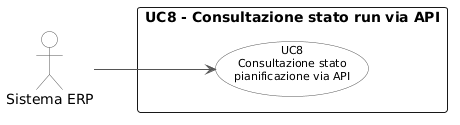
\includegraphics[width=0.75\columnwidth]{img/usecase/uc8.png}
    \caption{UC8 -- Stima ATP per nuovo ordine}
    \label{fig:uc8}
\end{figure}

\subsubsection{Consultazione stato pianificazione via API}

\paragraph{UC9 -- Consultazione stato pianificazione via API}
\begin{itemize}
    \item \textbf{Attore principale:} Sistema ERP.
    \item \textbf{Scenario principale:}
    \begin{enumerate}
        \item Il Sistema ERP invia una richiesta HTTP GET all'endpoint \texttt{/api/planning/status/\{run\_id\}} con l'identificativo del run ricevuto in UC2.B.
        \item Il server restituisce lo stato corrente del run (\texttt{Queued}, \texttt{Running}, \texttt{Finished} o \texttt{Failed}) e i KPI disponibili (makespan, lateness, numero di task schedulati).
        \item Se il run è ancora in corso, il Sistema ERP ripete la richiesta dopo un intervallo fino al completamento.
        \item Quando lo stato è \texttt{Finished}, il Sistema ERP elabora i dati del piano ricevuti nella risposta.
    \end{enumerate}
    \item \textbf{Precondizioni:}
    \begin{itemize}
        \item il server HTTP è disponibile e raggiungibile.
        \item il Sistema ERP dispone del \texttt{run\_id} ottenuto in UC2.B.
    \end{itemize}
    \item \textbf{Postcondizioni:}
    \begin{itemize}
        \item il Sistema ERP ha ricevuto lo stato aggiornato e i KPI del run.
    \end{itemize}
    \item \textbf{Trigger:} il Sistema ERP vuole verificare l'avanzamento o il completamento di una pianificazione avviata via API.
\end{itemize}

\begin{figure}[H]
    \centering
    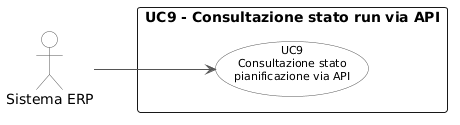
\includegraphics[width=0.65\columnwidth]{img/usecase/uc9.png}
    \caption{UC9 -- Consultazione stato pianificazione via API}
    \label{fig:uc9}
\end{figure}

\newpage

\section{Tracciamento dei requisiti}

A partire dall'analisi dei casi d'uso è stato definito un insieme di requisiti funzionali, qualitativi e di vincolo. Il codice identificativo dei requisiti segue la notazione riportata di seguito.

\begin{itemize}
    \item \textbf{F} -- Requisito funzionale
    \item \textbf{Q} -- Requisito qualitativo
    \item \textbf{V} -- Requisito di vincolo
    \item \textbf{N} -- Obbligatorio
    \item \textbf{D} -- Desiderabile
    \item \textbf{Z} -- Facoltativo
\end{itemize}

Tutti i requisiti riportati in questa sezione sono classificati come obbligatori; per questo motivo il codice termina con la lettera \textbf{N}.

\section{Tabelle dei requisiti}

\subsection{Requisiti funzionali}

\begin{center}
\rowcolors{1}{}{tableGray}
\begin{longtable}{|p{2.1cm}|p{6.9cm}|p{2.0cm}|p{2.0cm}|}
\hline
\multicolumn{1}{|c|}{\textbf{Requisito}} &
\multicolumn{1}{c|}{\textbf{Descrizione}} &
\multicolumn{1}{c|}{\textbf{Use Case}} &
\multicolumn{1}{c|}{\textbf{Necessità}} \\
\hline
\endfirsthead

\hline
\multicolumn{4}{c}{{\bfseries Continuazione della tabella}}\\
\hline
\multicolumn{1}{|c|}{\textbf{Requisito}} &
\multicolumn{1}{c|}{\textbf{Descrizione}} &
\multicolumn{1}{c|}{\textbf{Use Case}} &
\multicolumn{1}{c|}{\textbf{Necessità}} \\
\hline
\endhead

RFN-1  & Configurazione dei parametri di pianificazione & UC1 & N \\
\hline
RFN-2  & Inserimento della data di inizio pianificazione & UC1.1 & N \\
\hline
RFN-3  & Inserimento del timeout del solver & UC1.2 & N \\
\hline
RFN-4  & Selezione della strategia di risoluzione & UC1.3 & N \\
\hline
RFN-5  & Avvio della pianificazione & UC2 & N \\
\hline
RFN-6  & Monitoraggio dell'esecuzione del solver & UC3 & N \\
\hline
RFN-7  & Consultazione log di esecuzione & UC3.1 & N \\
\hline
RFN-8  & Consultazione KPI in tempo reale & UC3.2 & N \\
\hline
RFN-9  & Consultazione telemetria del solver & UC3.3 & N \\
\hline
RFN-10 & Consultazione dei risultati della pianificazione & UC4 & N \\
\hline
RFN-11 & Visualizzazione del diagramma di Gantt & UC4.1 & N \\
\hline
RFN-12 & Visualizzazione dei task pianificati & UC4.2 & N \\
\hline
RFN-13 & Analisi della qualità del piano & UC4.3 & N \\
\hline
RFN-14 & Esportazione del piano in formato JSON & UC5 & N \\
\hline
RFN-15 & Consultazione dell'elenco storico pianificazioni & UC6.1 & N \\
\hline
RFN-16 & Consultazione del dettaglio di esecuzioni storiche & UC6.2 & N \\
\hline
RFN-17 & Modifica delle priorità operative & UC7 & N \\
\hline
RFN-18 & Stima ATP per nuovi ordini & UC8 & N \\
\hline
RFN-19 & Selezione della modalità di esecuzione del solver (locale o remota via gRPC) & UC1.4 & N \\
\hline
RFN-20 & Avvio della pianificazione da interfaccia Qt & UC2.A & N \\
\hline
RFN-21 & Avvio della pianificazione tramite API HTTP da parte del Sistema ERP & UC2.B & N \\
\hline
RFN-22 & Consultazione dello stato e dei KPI di un run via API HTTP & UC9 & N \\
\hline

\caption{Tabella del tracciamento dei requisiti funzionali.}
\label{tab:requisiti_funzionali}
\end{longtable}
\end{center}

\subsection{Requisiti qualitativi}

\begin{center}
\rowcolors{1}{}{tableGray}
\begin{longtable}{|p{2.1cm}|p{6.9cm}|p{2.0cm}|p{2.0cm}|}
\hline
\multicolumn{1}{|c|}{\textbf{Requisito}} &
\multicolumn{1}{c|}{\textbf{Descrizione}} &
\multicolumn{1}{c|}{\textbf{Use Case}} &
\multicolumn{1}{c|}{\textbf{Necessità}} \\
\hline
\endfirsthead
\hline
\multicolumn{4}{c}{{\bfseries Continuazione della tabella}}\\
\hline
\endhead

RQN-1 & L'interfaccia deve risultare intuitiva e utilizzabile dagli operatori & UC1--UC8 & N \\
\hline
RQN-2 & Il sistema deve garantire tempi di risposta adeguati nella visualizzazione dei risultati & UC4 & N \\
\hline
RQN-3 & Le informazioni di esecuzione devono essere aggiornate in modo continuo durante il calcolo & UC3 & N \\
\hline
RQN-4 & La pianificazione deve rispettare i vincoli del modello di schedulazione & UC2 & N \\
\hline
RQN-5 & I dati esportati devono essere compatibili con strumenti esterni & UC5 & N \\
\hline
RQN-6 & Le esecuzioni devono essere tracciabili nello storico locale & UC6.1, UC6.2 & N \\
\hline

\caption{Tabella del tracciamento dei requisiti qualitativi.}
\label{tab:requisiti_qualitativi}
\end{longtable}
\end{center}

\subsection{Requisiti di vincolo}

\begin{center}
\rowcolors{1}{}{tableGray}
\begin{longtable}{|p{2.1cm}|p{6.9cm}|p{2.0cm}|p{2.0cm}|}
\hline
\multicolumn{1}{|c|}{\textbf{Requisito}} &
\multicolumn{1}{c|}{\textbf{Descrizione}} &
\multicolumn{1}{c|}{\textbf{Use Case}} &
\multicolumn{1}{c|}{\textbf{Necessità}} \\
\hline
\endfirsthead
\hline
\multicolumn{4}{c}{{\bfseries Continuazione della tabella}}\\
\hline
\endhead

RVN-1 & Il sistema deve essere sviluppato in linguaggio C++ & -- & N \\
\hline
RVN-2 & L'interfaccia grafica di debug e testing deve essere realizzata con Qt6 & -- & N \\
\hline
RVN-3 & Il solver di pianificazione deve utilizzare Google OR-Tools & UC2 & N \\
\hline
RVN-4 & L'esportazione dei dati deve avvenire in formato JSON & UC5 & N \\
\hline
RVN-5 & Lo storico locale deve essere persistito tramite SQLite & UC6.1, UC6.2 & N \\
\hline
RVN-6 & L'interfaccia HTTP di produzione deve essere realizzata con il framework Drogon & UC2.B & N \\
\hline

\caption{Tabella del tracciamento dei requisiti di vincolo.}
\label{tab:requisiti_vincolo}
\end{longtable}
\end{center}
